
\todo[inline]{cite main text figure for conformal transformation}
In the course of derivation the free energy subject to various boundary conditions, we use conformal transformation to convert the space time diagram with slits to a cylinder diagram, where the boundary state (and ground state energy calculation in App.~\ref{app:gnd_dn_lambda}) is applicable. However, free energy, especially its constant part, is not invariant under the conformal transformation, because the boundaries partially break the conformal symmetry. In this Appendix, we point out two corrections -- one from the outer boundary and the other from the inhomogeneous Schwartzian term -- to get the correct exponent of the fidelity and Loschmidt echo. 

% outer boundary correction
It is discussed in the pioneering work\cite{cardy_finite-size_1988} by Cardy and Peschel that boundary will contribute logarithmic term, which manifest itself as the geodesic curvature integral in the trace anomaly. Here we demonstrate this principle using the disk free energy example in Ref.~\cite{cardy_finite-size_1988}. Consider an annulus on flat space with inner radius $r_1$ and outer radius $r_2$. Its free energy is
\begin{equation}
F({\rm annulus}) = -  \frac{c}{6} \ln \frac{r_2}{r_1} 
\end{equation}
On the other hand the free energy of a disk of radius $r_2$ is
\begin{equation}
  F( {\rm disk} ) = - \frac{c}{6} \ln \frac{r_2}{a}
\end{equation}
where $a$ is the short distance regulator. The disk free energy is completely contributed by its outer boundary and so the one can interpret the annulus free energy as the additive contribution from its outer and inner surfaces (which is also consistent with the geodesic curvature integral calculation),
\begin{equation}
F( {\rm annulus} ) = -  \frac{c}{6} \ln \frac{r_2}{a} +  \frac{c}{6} \ln \frac{r_1}{a} = - \frac{c}{6} \ln \frac{r_2}{r_1}
\end{equation}
An annulus becomes a disk when its inner radius is of order $a$, and we can see that the contribution from the inner surface $\frac{c}{6} \ln \frac{r_1}{a}$ becomes negligible. 

\todo[inline]{citing figure}
We now scrutinize the conformation transformation from the slit diagram to the annulus. In the slit diagram, the regulators all have radius that is order of the short distance cut-off. They will have negligible contributions to the free energy. However, after doing the conformal transformation (passive), the outer surface will contribute $-\frac{c}{6} \ln \frac{r_2}{r_1}$ which should not be there. Using the parameters in the free energy calculation in other appendices, we have 
\begin{equation}
F_{\xi } = F_{z} + \frac{c}{6} \beta 
\end{equation}

% staircase geometry correction
The annulus is called staircase geometry Ref.~\onlinecite{cardy_finite-size_1988} due to its angular direction of time evolution. The traditional radial quantization however has radial direction to be the time direction. One can go through a series of conformal maps, one can show that that the Hamiltonian of the staircase and rectangle has a shift due to the Schwartzian
\begin{equation}
H_{z} = H_{\xi} - \frac{c}{24\pi} \beta 
\end{equation}
After the evolution for $2\pi$, the difference in the free energy is
\begin{equation}
F_w = F_{\xi} - \frac{c}{12} \beta 
\end{equation}
Gathering the two together, we obtain the missing $\frac{c}{12} \beta$ between the echo diagram and the Casimir energy, 
\begin{equation}
F_{w} = F_z + {\color{red} \frac{c}{12}\beta }
\end{equation}
\begin{figure}[h]
\centering
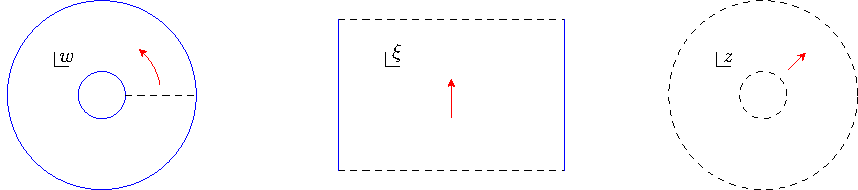
\includegraphics[width=\textwidth]{fig_uncon_rq.pdf}
\caption{Unconventional radial quantization on annulus(torus). Left panel: unlike the conventional radial quantization, we view the dashed line as a state and to time evolution in the radial direction. The blue circles are regarded as boundaries conditions rather than asymptotic states. Middle panel: $\xi = \ln w$ plane. Right panel: $z = \exp(i \frac{2\pi}{\beta} \xi)$ plane. We treat those dashed lines as asymptotic states and perform standard radial quantization here.}
\label{fig:uncon_rq}
\end{figure}

\todo[inline]{There are two series of conformal transformation, one is the main text, the other is the staircase geometry. Both use $w, z, \xi$, I will fix the notation after the main text figure is complete. Maybe detailed computation of the Schwartzian term is necessary, because of the sign. }

%%% Local Variables:
%%% TeX-master: "bCFT_paper"
%%% TeX-PDF-mode: t
%%% End:
